%
% packets.tex
%
% Copyright The FloripaSat-2 Contributors.
%
% FloripaSat-2 Documentation
%
% This work is licensed under the Creative Commons Attribution-ShareAlike 4.0
% International License. To view a copy of this license,
% visit http://creativecommons.org/licenses/by-sa/4.0/.
%

%
% \brief EDC test report appendix.
%
% \author Gabriel Mariano Marcelino <gabriel.mm8@gmail.com>
%
% \version 0.9.0
%
% \date 2022/03/12
%

\chapter{EDC Test Report} \label{anx:edc-report}

This appendix is a test report of the EDC board. The purpose of this test is to characterize the main functionalities of the EDC module. The main information about the test are available below:

\begin{itemize}
    \item \textbf{Date}: From 2022/03/03 to 2022/03/14
    \item \textbf{Testers}: Bruno Benedetti, Gabriel M. Marcelino, Laio O. Seman
\end{itemize}

A picture of the boards used during the tests can be seen in \autoref{fig:edc-boards-test}.

\begin{figure}[!htb]
    \begin{center}
        \subfigure[Top side.\label{fig:edc-top-test}]{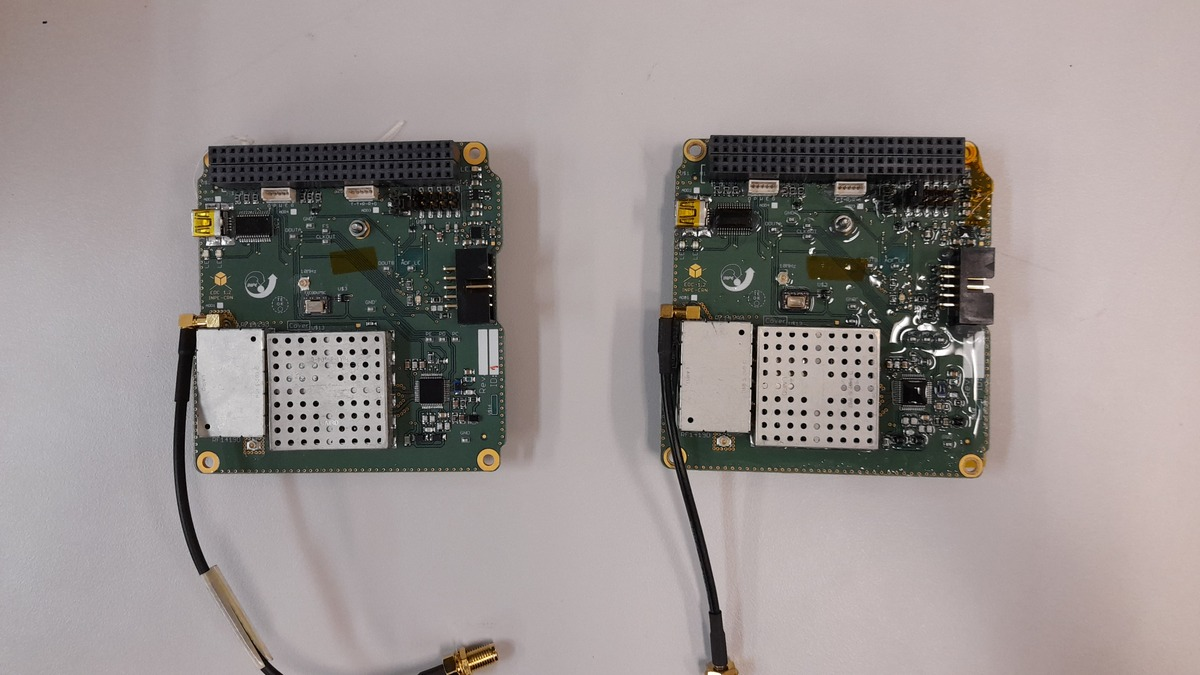
\includegraphics[width=\textwidth]{figures/edc_report/edcs-top}}

        \subfigure[Bottom side.\label{fig:edc-bottom-test}]{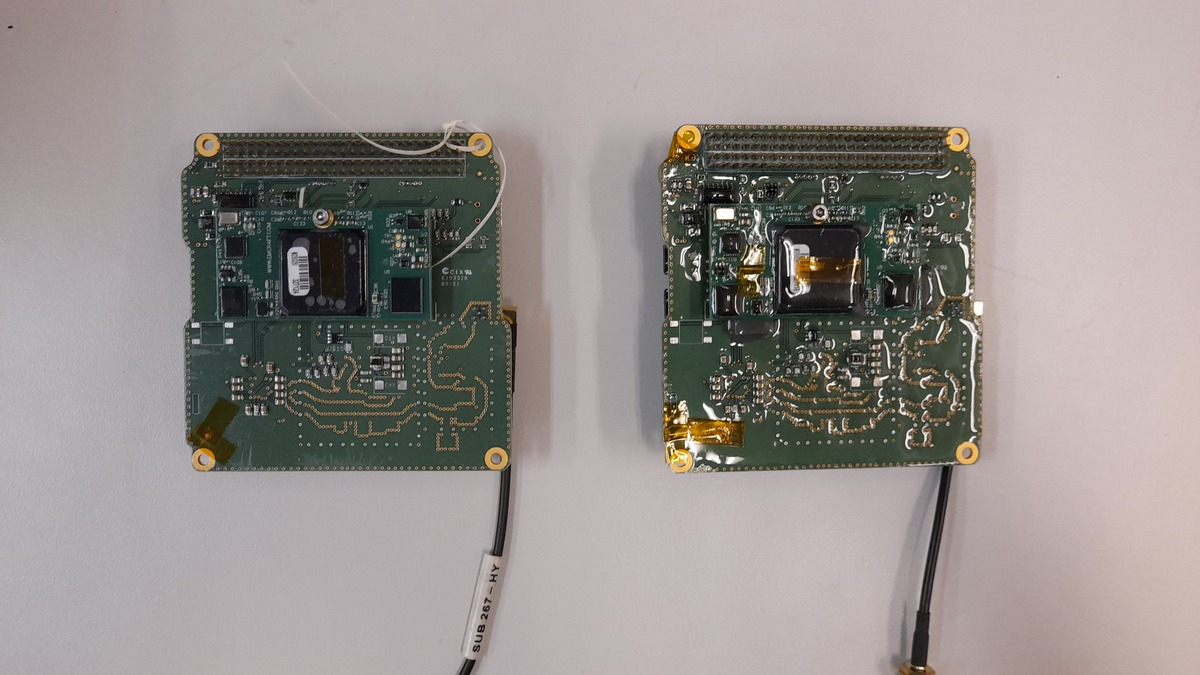
\includegraphics[width=\textwidth]{figures/edc_report/edcs-bottom}}
        \caption{Tested EDC boards.}
        \label{fig:edc-boards-test}
    \end{center}
\end{figure}

This test is divided in two parts: command interface test, and RF chain test. Both are described below.

\section{Command interface test}

The command interface test has the purpose of testing the UART command interface available in the PC-104 bus of the module. All available commands were tested in this test.

\subsection{Used material}

The used material is listed below:

\begin{itemize}
    \item EDC boards
    \item USB-UART converter
    \item Saleae Logic Analyzer
    \item Protoboard
    \item Desktop computer
    \item Logic 2 software
    \item Cutecom software
    \item USB cables
    \item Pin header wires
    \item EDC documentation
\end{itemize}

\subsection{Setup}

The setup of the test can be seen in \autoref{fig:edc-test-setup}. As can be seen in the picture, the USB-UART converter connects the UART interface of the EDC directly to a computer. The EDC board is powered directly by its USB debug interface.

\begin{figure}[!ht]
    \begin{center}
        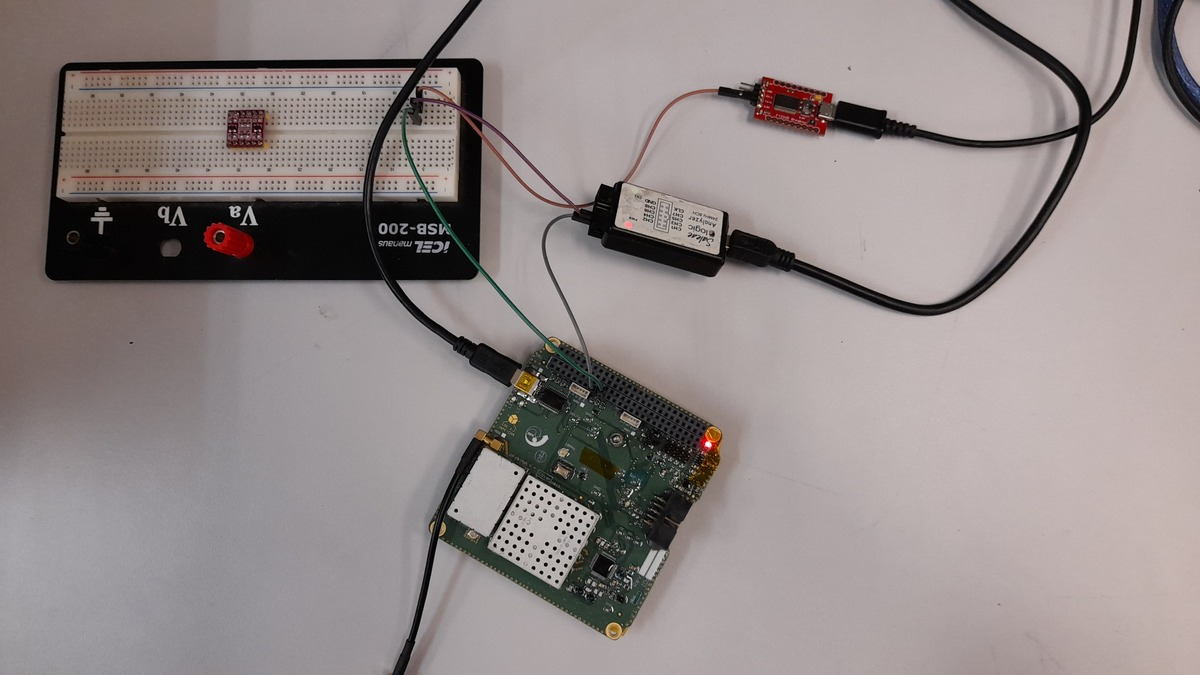
\includegraphics[width=\textwidth]{figures/edc_report/cmd-test-setup}
        \caption{Setup of the EDC's command interface test.}
        \label{fig:edc-test-setup}
    \end{center}
\end{figure}

To confirm and visualize the transmitted and received data, a logic analyzer is connected to the pins of the UART interface (TX and RX).

\subsection{Results}

During the first attempts to perform this test, no response were received from both boards, during all available commands. After further investigation with the developers of the module (INPE-CRN), the issue was found. As can be seen in autoref{fig:edc-cmd-issue}, the voltage of the RX pin when in low state is higher than expected, making all bits be interpreted as ones.

\begin{figure}[!ht]
    \begin{center}
        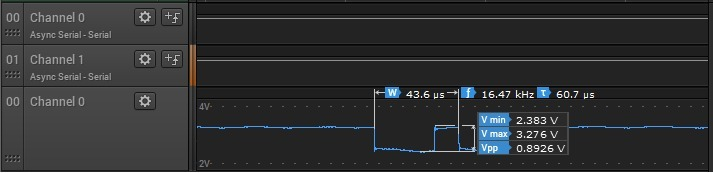
\includegraphics[width=\textwidth]{figures/edc_report/edc-cmd-issue}
        \caption{Command interface issue.}
        \label{fig:edc-cmd-issue}
    \end{center}
\end{figure}

The hypothesis for the cause of this problem is the RS-485 transceiver. As can be seen in \autoref{fig:edc-bd-uart-if}, the RS-485 transceiver and the UART interfaces shares the same UART port of the microcontroller. This way, the RS-485 transceiver can cause an interference on the RX pin of the UART interface, forcing its state to high all the time.

\begin{figure}[!ht]
    \begin{center}
        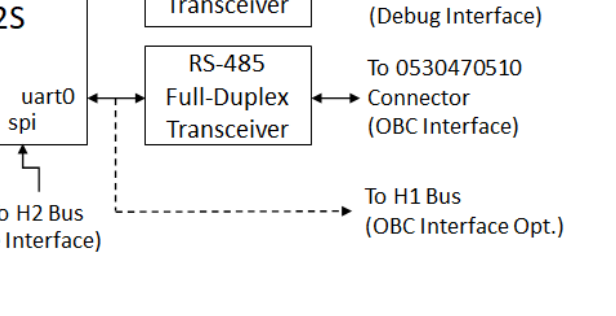
\includegraphics[width=0.6\textwidth]{figures/edc_report/edc-bd-uart-if}
        \caption{UART and RS-485 interfaces of the EDC.}
        \label{fig:edc-bd-uart-if}
    \end{center}
\end{figure}

A solution to this problem, is to disable the RS-485 transceiver, by removing it from the board, or putting the enable pin on disabled state. As it would be difficult to safety remove this component from the boards, the second option was chosen. With a modification in the firmware, the RS-485 transceiver was disabled, and after this modification, the UART command interface started to work as expected, as can be seen in \autoref{fig:edc-echo-cmd} (``echo'' command).

\begin{figure}[!ht]
    \begin{center}
        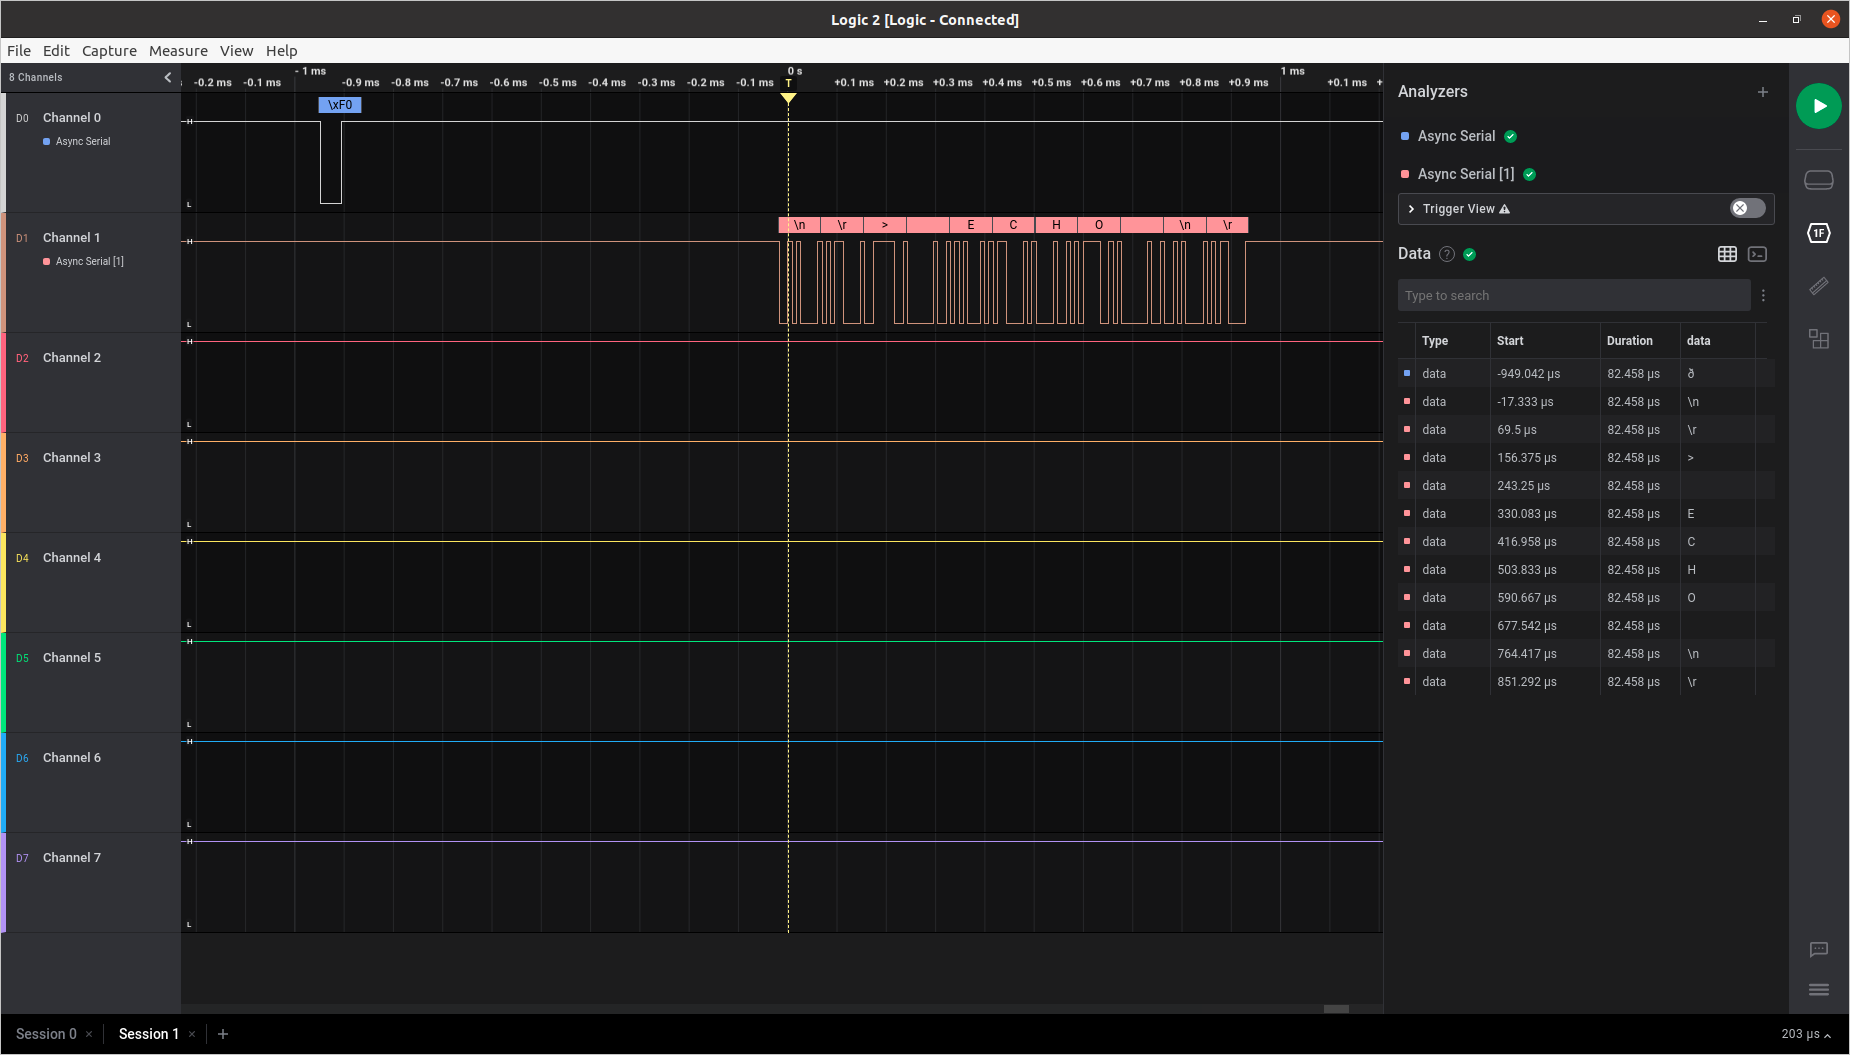
\includegraphics[width=\textwidth]{figures/edc_report/echo-cmd}
        \caption{``Echo'' command demonstration.}
        \label{fig:edc-echo-cmd}
    \end{center}
\end{figure}

\section{RF chain test}

This test simulates a signal transmitted by a DCP directly to the RF input of the EDC module. To emulate the DCP signal, a GNURadio flow generates the packets and an SDR transmitted transmits the packet to the EDC. This test is divided in two steps: in the first step, we check the transmitted signal by the USRP, and in the second step the EDC reception and decoding is verified.

\subsection{Used material}

The used material is listed below:

\begin{itemize}
    \item EDC boards
    \item USB-UART converter
    \item Ettus USRP B210 SDR
    \item Desktop computer
    \item GNURadio v3.9
    \item Cutecom software
    \item USB cables
    \item Pin header wires
    \item SMA coaxial cable
    \item 30 dB attenuator
    \item RTL-SDR v3
    \item EDC documentation
\end{itemize}

\subsection{Setup}

This test is divided in two steps. The setup of the first step can be seen in \autoref{fig:edc-stimulus-test}. As can be seen in the picture, the SDR transmitter is connected directly to an SDR receiver through a 30 dB attenuator.

\begin{figure}[!ht]
    \begin{center}
        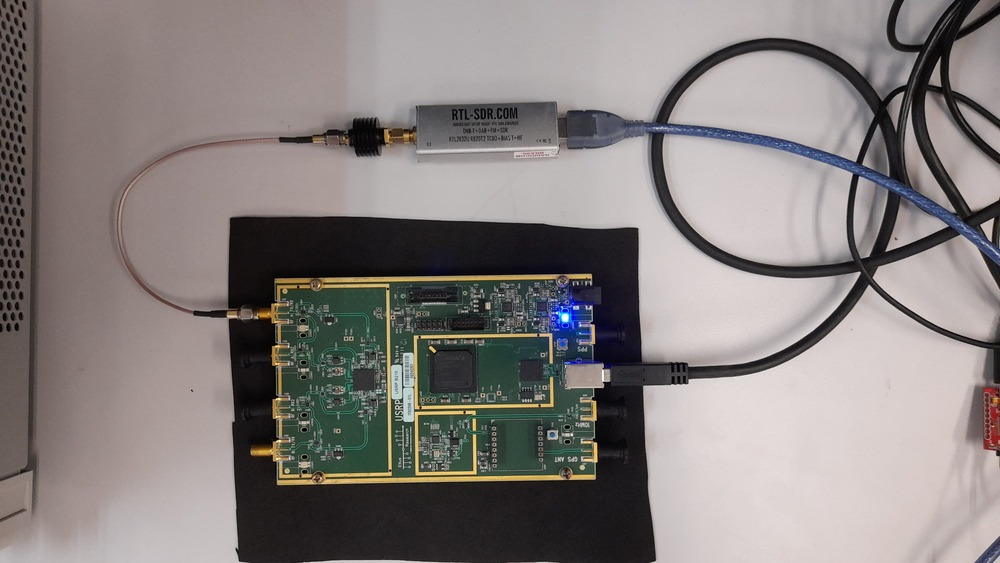
\includegraphics[width=\textwidth]{figures/edc_report/edc-stimulus-test}
        \caption{Setup of the signal generator test.}
        \label{fig:edc-stimulus-test}
    \end{center}
\end{figure}

\begin{figure}[!ht]
    \begin{center}
        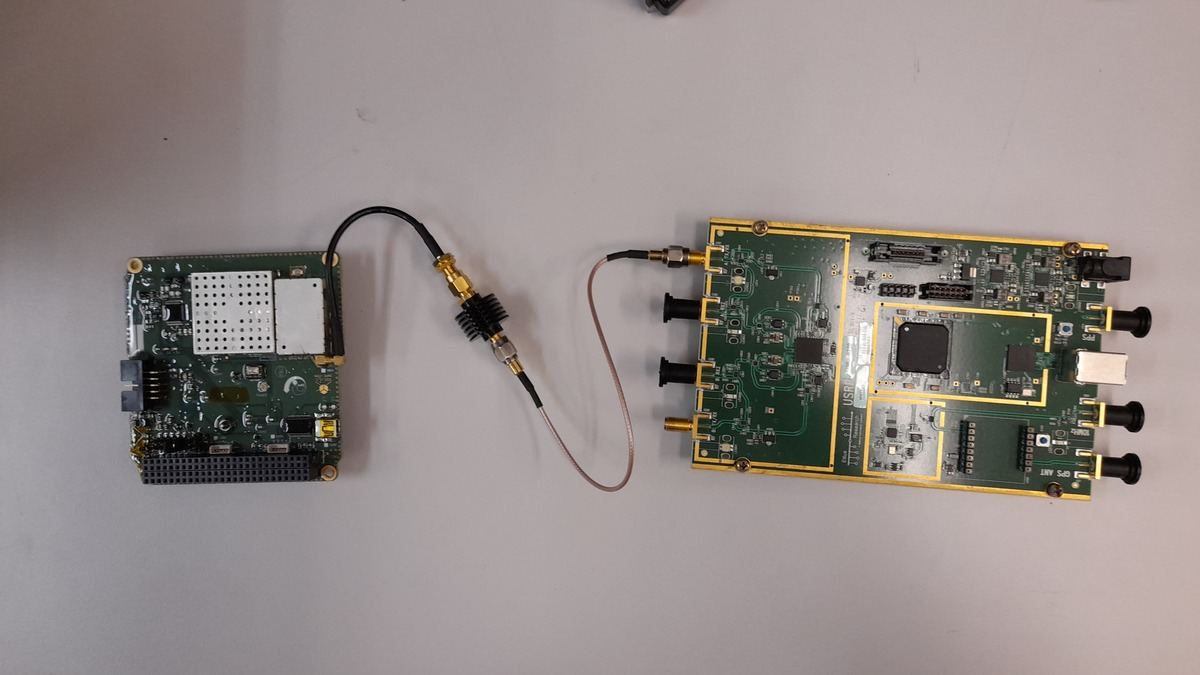
\includegraphics[width=\textwidth]{figures/edc_report/rf-chain-setup}
        \caption{Setup of the EDC's RF chain test.}
        \label{fig:edc-rf-chain-test-setup}
    \end{center}
\end{figure}

\begin{figure}[!ht]
    \begin{center}
        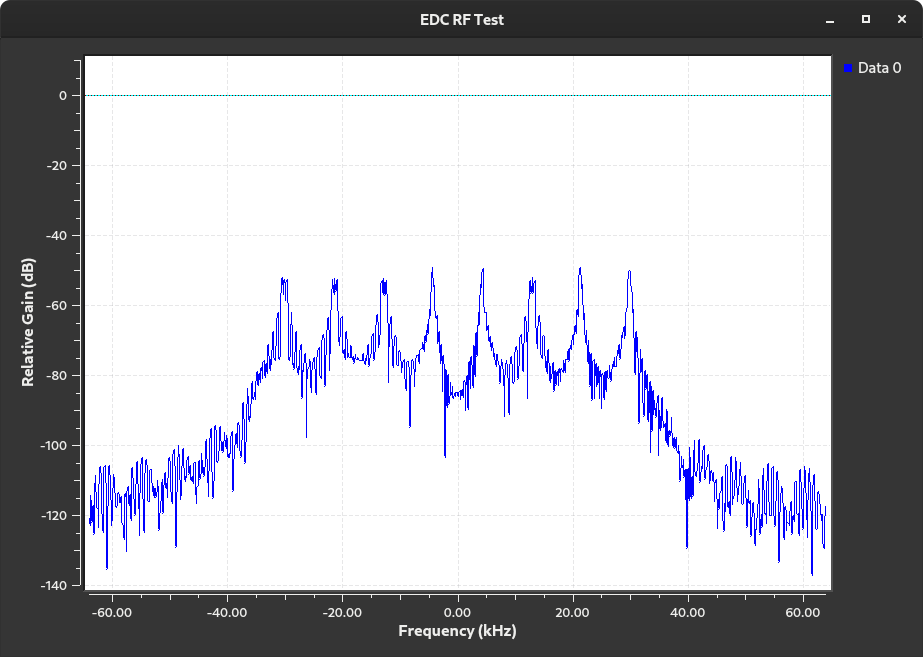
\includegraphics[width=\textwidth]{figures/edc_report/edc-rf-test-signal}
        \caption{Generated signal used in the RF chain test.}
        \label{fig:edc-rf-signal}
    \end{center}
\end{figure}

\subsection{Results}

The transmitted signal by the USRP SDR can be seen in \autoref{fig:edc-rf-signal-gqrx}.

\begin{figure}[!ht]
    \begin{center}
        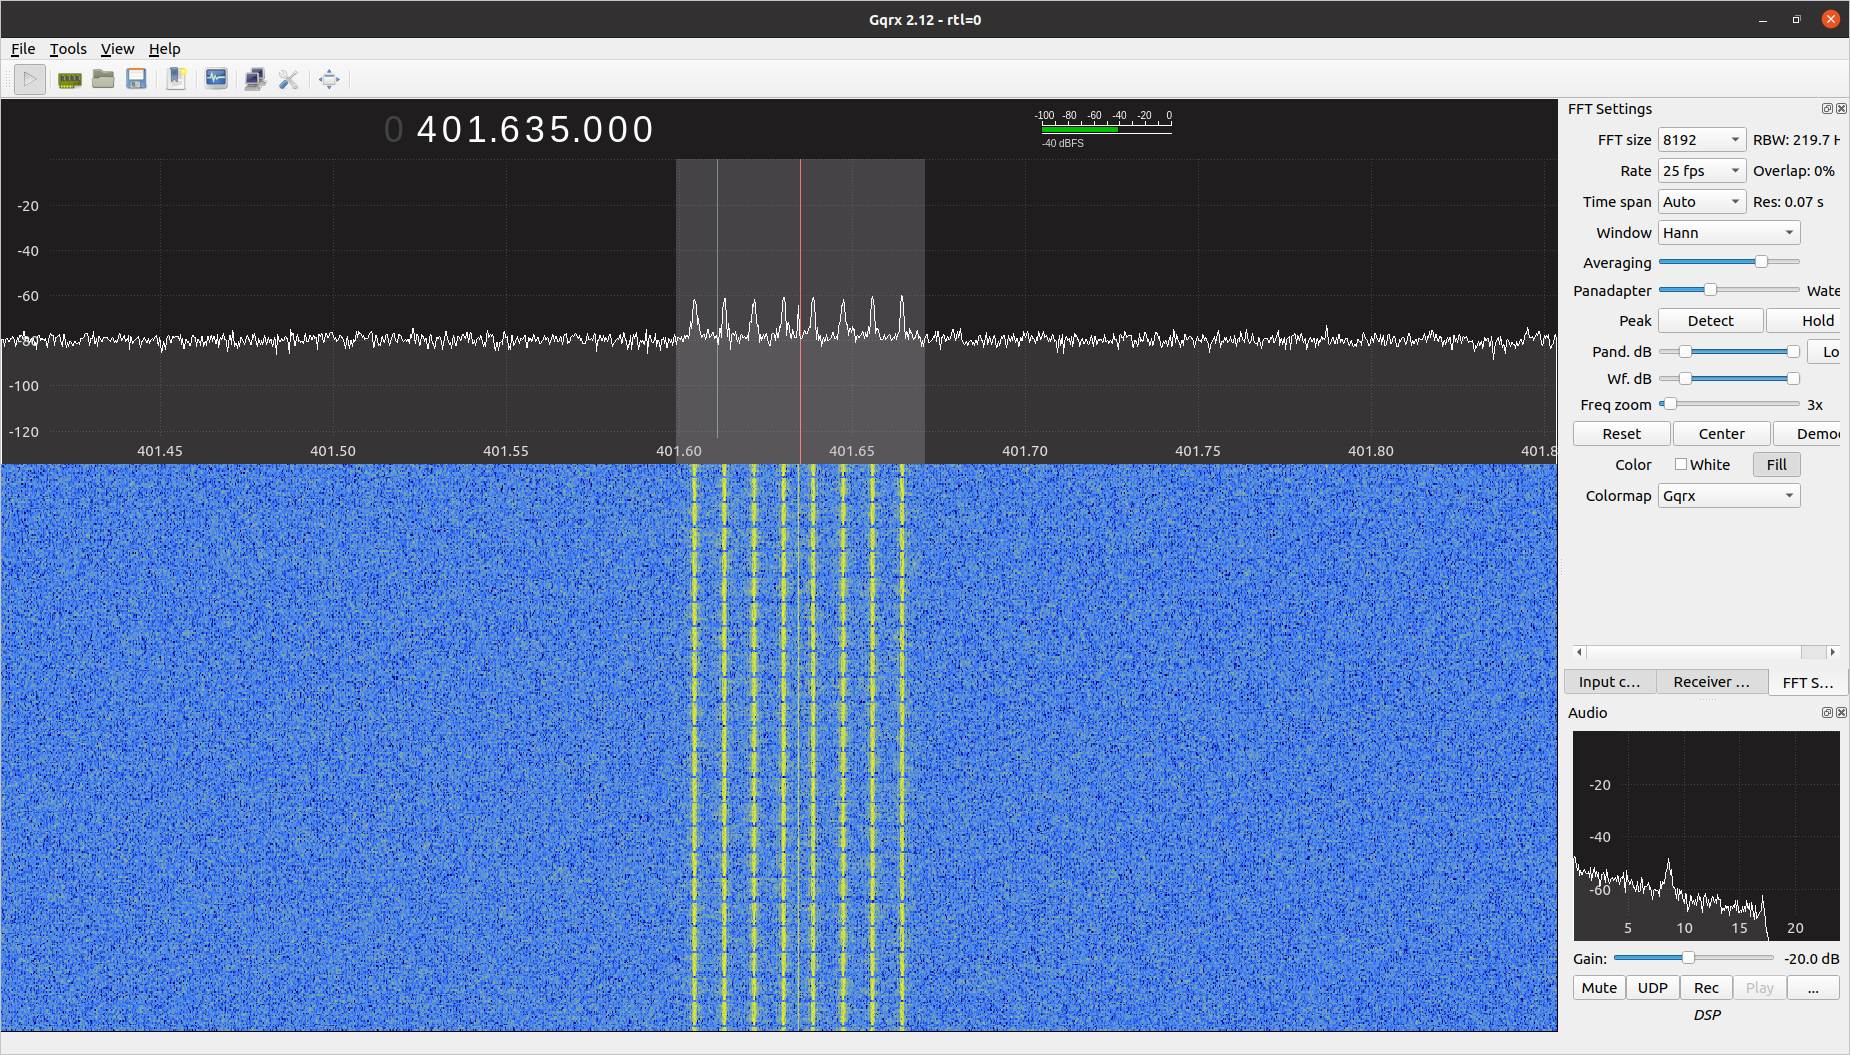
\includegraphics[width=\textwidth]{figures/edc_report/edc-stimulus}
        \caption{Received signal from the EDC stimulus application.}
        \label{fig:edc-rf-signal-gqrx}
    \end{center}
\end{figure}

The received and decoded packets by the EDC during the tests, are available in \autoref{fig:edc-pkts}. Each color line is a different decoded packet. The last byte sequence indicates the number of available packets in the queue (zero in this case, after reading all packets).

\begin{figure}[!ht]
    \begin{center}
        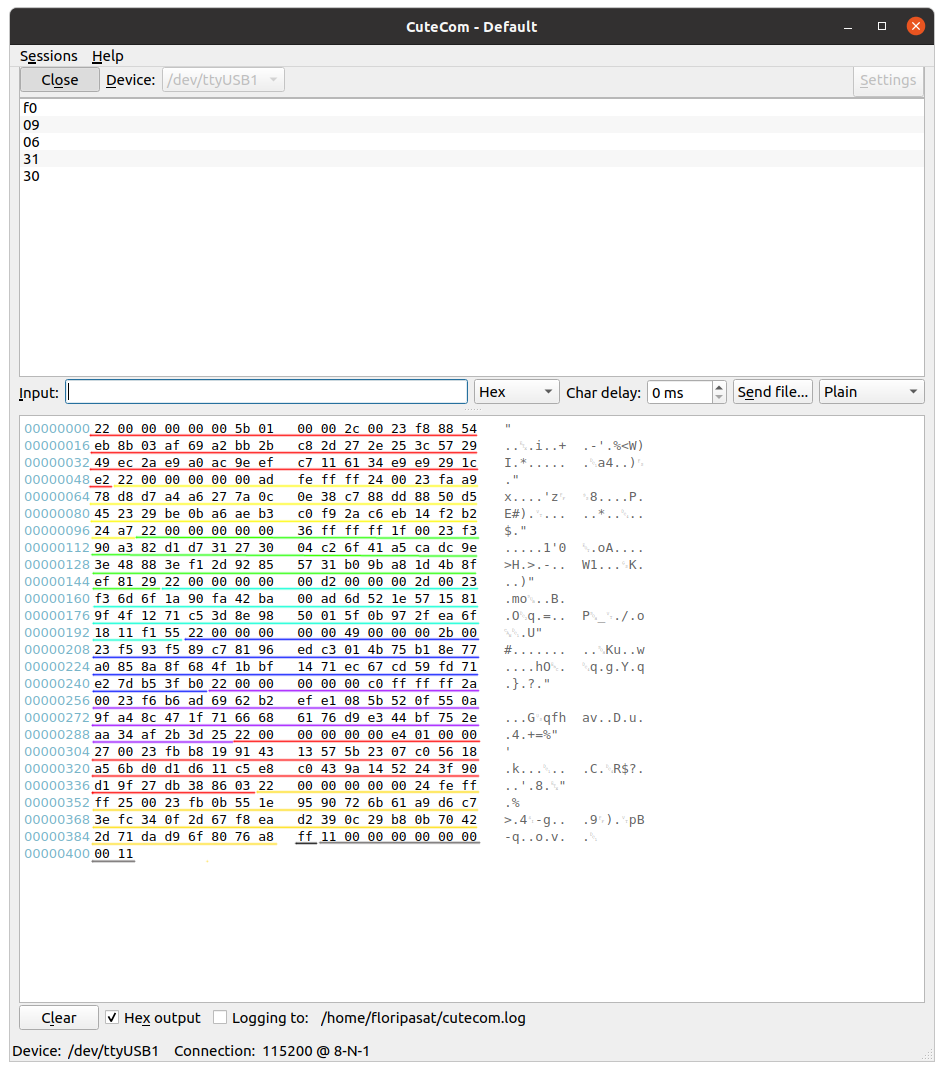
\includegraphics[width=0.8\textwidth]{figures/edc_report/ptt-pkg}
        \caption{Received PTT packages (colorful lines).}
        \label{fig:edc-pkts}
    \end{center}
\end{figure}

\section{Conclusion}

As presented on this report, a issue with the UART interface was found. A temporary solution was achieved by modifying the current version of the firmware, disabling the RS-485 transceiver by software. But, for the flight version of the boards, a better solution should be considered, per example, the RS-485 CI can be unconsidered from the board assembly or disabled by hardware (with a jumper).

As for the RF chain test, no issues were identified so far, using the available stimulus signal, all packages are received and decoded as expected. The commands regarding the package reception also work as planned.
